% Options for packages loaded elsewhere
\PassOptionsToPackage{unicode}{hyperref}
\PassOptionsToPackage{hyphens}{url}
\PassOptionsToPackage{dvipsnames,svgnames,x11names}{xcolor}
%
\documentclass[
]{article}

\usepackage{amsmath,amssymb}
\usepackage{iftex}
\ifPDFTeX
  \usepackage[T1]{fontenc}
  \usepackage[utf8]{inputenc}
  \usepackage{textcomp} % provide euro and other symbols
\else % if luatex or xetex
  \usepackage{unicode-math}
  \defaultfontfeatures{Scale=MatchLowercase}
  \defaultfontfeatures[\rmfamily]{Ligatures=TeX,Scale=1}
\fi
\usepackage{lmodern}
\ifPDFTeX\else  
    % xetex/luatex font selection
\fi
% Use upquote if available, for straight quotes in verbatim environments
\IfFileExists{upquote.sty}{\usepackage{upquote}}{}
\IfFileExists{microtype.sty}{% use microtype if available
  \usepackage[]{microtype}
  \UseMicrotypeSet[protrusion]{basicmath} % disable protrusion for tt fonts
}{}
\usepackage{xcolor}
\setlength{\emergencystretch}{3em} % prevent overfull lines
\setcounter{secnumdepth}{-\maxdimen} % remove section numbering
% Make \paragraph and \subparagraph free-standing
\ifx\paragraph\undefined\else
  \let\oldparagraph\paragraph
  \renewcommand{\paragraph}[1]{\oldparagraph{#1}\mbox{}}
\fi
\ifx\subparagraph\undefined\else
  \let\oldsubparagraph\subparagraph
  \renewcommand{\subparagraph}[1]{\oldsubparagraph{#1}\mbox{}}
\fi


\providecommand{\tightlist}{%
  \setlength{\itemsep}{0pt}\setlength{\parskip}{0pt}}\usepackage{longtable,booktabs,array}
\usepackage{calc} % for calculating minipage widths
% Correct order of tables after \paragraph or \subparagraph
\usepackage{etoolbox}
\makeatletter
\patchcmd\longtable{\par}{\if@noskipsec\mbox{}\fi\par}{}{}
\makeatother
% Allow footnotes in longtable head/foot
\IfFileExists{footnotehyper.sty}{\usepackage{footnotehyper}}{\usepackage{footnote}}
\makesavenoteenv{longtable}
\usepackage{graphicx}
\makeatletter
\def\maxwidth{\ifdim\Gin@nat@width>\linewidth\linewidth\else\Gin@nat@width\fi}
\def\maxheight{\ifdim\Gin@nat@height>\textheight\textheight\else\Gin@nat@height\fi}
\makeatother
% Scale images if necessary, so that they will not overflow the page
% margins by default, and it is still possible to overwrite the defaults
% using explicit options in \includegraphics[width, height, ...]{}
\setkeys{Gin}{width=\maxwidth,height=\maxheight,keepaspectratio}
% Set default figure placement to htbp
\makeatletter
\def\fps@figure{htbp}
\makeatother

\usepackage{booktabs}
\usepackage{longtable}
\usepackage{array}
\usepackage{multirow}
\usepackage{wrapfig}
\usepackage{float}
\usepackage{colortbl}
\usepackage{pdflscape}
\usepackage{tabu}
\usepackage{threeparttable}
\usepackage{threeparttablex}
\usepackage[normalem]{ulem}
\usepackage{makecell}
\usepackage{xcolor}
\usepackage[noblocks]{authblk}
\renewcommand*{\Authsep}{, }
\renewcommand*{\Authand}{, }
\renewcommand*{\Authands}{, }
\renewcommand\Affilfont{\small}
\usepackage{caption}
\DeclareCaptionLabelFormat{Sformat}{#1 S1-#2}
\captionsetup[table]{labelformat=Sformat}
\captionsetup[figure]{labelformat=Sformat}
\usepackage{mathtools}
\usepackage[sort, round]{natbib}
\usepackage[left]{lineno}
\usepackage{tabularx}
\linenumbers
\usepackage[a4paper, total={6in, 10in}]{geometry}
\usepackage{longtable}
\usepackage[colorlinks=true,linkcolor=black,citecolor=black,urlcolor=black]{hyperref}
\usepackage{amsmath,amssymb,amsfonts,amsthm}
\usepackage{multirow}
\usepackage{setspace}\doublespacing
\renewcommand{\abstractname}{Summary}
\usepackage{bm}
\usepackage{algorithm}
\usepackage{algpseudocode}
\usepackage{rotating}
\makeatletter
\makeatother
\makeatletter
\makeatother
\makeatletter
\@ifpackageloaded{caption}{}{\usepackage{caption}}
\AtBeginDocument{%
\ifdefined\contentsname
  \renewcommand*\contentsname{Table of contents}
\else
  \newcommand\contentsname{Table of contents}
\fi
\ifdefined\listfigurename
  \renewcommand*\listfigurename{List of Figures}
\else
  \newcommand\listfigurename{List of Figures}
\fi
\ifdefined\listtablename
  \renewcommand*\listtablename{List of Tables}
\else
  \newcommand\listtablename{List of Tables}
\fi
\ifdefined\figurename
  \renewcommand*\figurename{Figure}
\else
  \newcommand\figurename{Figure}
\fi
\ifdefined\tablename
  \renewcommand*\tablename{Table}
\else
  \newcommand\tablename{Table}
\fi
}
\@ifpackageloaded{float}{}{\usepackage{float}}
\floatstyle{ruled}
\@ifundefined{c@chapter}{\newfloat{codelisting}{h}{lop}}{\newfloat{codelisting}{h}{lop}[chapter]}
\floatname{codelisting}{Listing}
\newcommand*\listoflistings{\listof{codelisting}{List of Listings}}
\makeatother
\makeatletter
\@ifpackageloaded{caption}{}{\usepackage{caption}}
\@ifpackageloaded{subcaption}{}{\usepackage{subcaption}}
\makeatother
\makeatletter
\@ifpackageloaded{tcolorbox}{}{\usepackage[skins,breakable]{tcolorbox}}
\makeatother
\makeatletter
\@ifundefined{shadecolor}{\definecolor{shadecolor}{rgb}{.97, .97, .97}}
\makeatother
\makeatletter
\makeatother
\makeatletter
\makeatother
\ifLuaTeX
  \usepackage{selnolig}  % disable illegal ligatures
\fi
\usepackage[]{natbib}
\bibliographystyle{plainnat}
\IfFileExists{bookmark.sty}{\usepackage{bookmark}}{\usepackage{hyperref}}
\IfFileExists{xurl.sty}{\usepackage{xurl}}{} % add URL line breaks if available
\urlstyle{same} % disable monospaced font for URLs
\hypersetup{
  pdftitle={Supplementary Information 1 : Integrating data from different taxonomic resolutions to better estimate community alpha diversity.},
  pdfauthor={Kwaku Peprah Adjei; Claire Carvell; Nick Isaac; Francesca Mancini; Robert B. O'Hara},
  colorlinks=true,
  linkcolor={black},
  filecolor={Maroon},
  citecolor={black},
  urlcolor={Blue},
  pdfcreator={LaTeX via pandoc}}

\title{Supplementary Information 1 : Integrating data from different
taxonomic resolutions to better estimate community alpha diversity.}


\author[1,2]{Kwaku Peprah Adjei}
\author[3]{Claire Carvell}
\author[3]{Nick Isaac}
\author[3]{Francesca Mancini}
\author[1,2]{Robert B. O'Hara}

\affil[1]{Department of Mathematical Sciences, Norwegian University of
Science and Technology, Trondheim Norway}
\affil[2]{Center for Biodiversity Dynamics, Norwegian University of
Science and Technology, Trondheim Norway}
\affil[3]{UK Center of Ecology and Hydrology, Wallingford UK}


\date{}
\begin{document}
\maketitle
\ifdefined\Shaded\renewenvironment{Shaded}{\begin{tcolorbox}[interior hidden, frame hidden, borderline west={3pt}{0pt}{shadecolor}, enhanced, breakable, boxrule=0pt, sharp corners]}{\end{tcolorbox}}\fi

\hypertarget{exploratory-analysis}{%
\section{Exploratory analysis}\label{exploratory-analysis}}

\hypertarget{introduction}{%
\subsection{Introduction}\label{introduction}}

An overlooked step in developing integrated distribution models is
exploring a model that fits each dataset. IDM takes advantage of the
shared parameters to get better inference, and is not an escape from
doing exploratory analysis on each dataset.

This supplementary material performs exploratory analysis on the UK
pollinator monitoring scheme \citep{breeze2021pollinator}. As mentioned
in the main paper, we have data from three insect groups: bumblebees,
solitary bees and hoverflies; and the models are fit independently for
each insect group. The exploration is therefore also done for each
insect group.

A Poisson and negative binomial generalised linear (mixed) models (GLMM
hereafter) were fit for each insect group in the group counts dataset
and binomial GLMM to the species occupancy data. The Poisson and
logistic regression are the simplest model to fit to the count and
occupancy data respectively \citep{fahrmeir2022regression}. When there
is overdispersion in the count data, the negative binomial regression
will fit the count data better \citep{fahrmeir2022regression}. The
negative binomial regression adds an extra parameter \(\phi\) to model
the extra variation in the data. Values of \(\phi\) closer to \(0\)
indicate overdispersion in the count data. A likelihood ratio test of
significance for the overdispersion parameter was performed. For each
insect group, the log-likelihoods from the Poisson and negative Binomial
regression models (\(l(\hat\beta_{NB})\) and \(l(\hat\beta_{Poi})\)
respectively) were retrieved and test statistic used was:

\[
LRT = -2 \times (l(\hat\beta_{NB}) - l(\hat\beta_{Poi})) \sim \chi^2_1.
\] The negative binomial distribution is chosen for the count data if
the p-value is less than \(0.05\) and Poisson is chosen when the p-value
if greater than \(0.05\).

We performed stepwise model selection technique to obtain the best model
for the count and occupancy data. We fit four models which we defined in
Equation~\ref{eq-models}: the first model \(M_{0}\) was an
intercept-only model; the second model \(M_{1}\) has an intercept and
latitudinal gradient as a covariate; the third model \(M_{2}\) added
visits as a random effect to model \(M_{1}\); and the last model
\(M_{3}\) added species as a random effect to model \(M_{2}\). Model
\(M_{3}\) was for the species occupancy data only, but the others were
for both datasets. We fit the models \(M_{0}\) and \(M_{1}\) with the
lme4 package \citep{bates2009package} and \(M_{2}\) and \(M_{3}\) with
the MASS package \citep{venables2022MASS} in R. The models were compared
using their BIC values. We chose BIC over AIC values because they have
high penalty for model complexity. The best model was the model with the
lowest BIC value.

\begin{equation}\protect\hypertarget{eq-models}{}{
\begin{split}
M_{0}&: \text{intercept} \\
M_{1}&: \text{intercept} + \text{latitude}\\
M_{2}&: \text{intercept}+ \text{latitude} + (1|visit)\\
M_{3}&: \text{intercept} + \text{latitude} + (1|visit) + (1|species)\\
\end{split}
}\label{eq-models}\end{equation}

\hypertarget{tbl-allModels}{}
\begin{table}
\caption{\label{tbl-allModels}Coefficients from the best models (model equations defined above for
BestModelIndex) for the group count and species occupancy data. The
BestModelIndex shows which of the model fitted were selected as the best
model (where best model is defined as the fitted model with the lowest
BIC value); the Intercept and Latitude are fixed effect estimates;
VisitVar and SpeciesVar are visit and species random effect variance
estimates respectively; Psi is the overdispersion parameter of the
negative Binomial and the P.value is the p-value estimate from
likelihood ratio test of overdispersion (the difference between the
Poisson and Negative Binomial models for each insect group). }\tabularnewline

\centering
\resizebox{\linewidth}{!}{
\begin{tabular}[t]{lllrrrrrr}
\toprule
Model & Data & BestModel & Intercept & Latitude & VisitVar & SpeciesVar & Psi & P.value\\
\midrule
\addlinespace[0.3em]
\multicolumn{9}{l}{\textbf{Bumblebees}}\\
\hspace{1em}\cellcolor{gray!6}{Binomial} & \cellcolor{gray!6}{Occupancy} & \cellcolor{gray!6}{M3} & \cellcolor{gray!6}{-4.54} & \cellcolor{gray!6}{0.08} & \cellcolor{gray!6}{0.07} & \cellcolor{gray!6}{1.95} & \cellcolor{gray!6}{-} & \cellcolor{gray!6}{-}\\
\hspace{1em}Negative Binomial & Counts & M1 & 0.14 & -0.38 & - & - & 1.42 & 0\\
\addlinespace[0.3em]
\hline
\multicolumn{9}{l}{\textbf{Hoverflies}}\\
\hspace{1em}\cellcolor{gray!6}{Binomial} & \cellcolor{gray!6}{Occupancy} & \cellcolor{gray!6}{M3} & \cellcolor{gray!6}{-5.16} & \cellcolor{gray!6}{0.23} & \cellcolor{gray!6}{0.02} & \cellcolor{gray!6}{2.70} & \cellcolor{gray!6}{-} & \cellcolor{gray!6}{-}\\
\hspace{1em}Negative Binomial & Counts & M2 & 0.96 & -0.13 & 0.03 & - & 1.36 & 0\\
\addlinespace[0.3em]
\hline
\multicolumn{9}{l}{\textbf{Solitarybees}}\\
\hspace{1em}\cellcolor{gray!6}{Binomial} & \cellcolor{gray!6}{Occupancy} & \cellcolor{gray!6}{M3} & \cellcolor{gray!6}{-5.99} & \cellcolor{gray!6}{-0.82} & \cellcolor{gray!6}{0.09} & \cellcolor{gray!6}{1.49} & \cellcolor{gray!6}{-} & \cellcolor{gray!6}{-}\\
\hspace{1em}Negative Binomial & Counts & M1 & -0.99 & -0.53 & - & - & 1.37 & 0\\
\bottomrule
\end{tabular}}
\end{table}

\hypertarget{results-and-interpretation}{%
\subsection{Results and
Interpretation}\label{results-and-interpretation}}

Figure~\ref{fig-bbGCPlot}, Figure~\ref{fig-hvGCPlot} and
Figure~\ref{fig-sbGCPlot} shows the distribution the bumblebees,
hoverflies and solitary bees group count data for each visit to the
\(74\) PoMS sites; Figure~\ref{fig-bbSOPlot}, Figure~\ref{fig-hvSOPlot}
and Figure~\ref{fig-sbSOPlot} shows the distribution of the proportion
of species occupying a given PoMS sites at each survey visit. The
Figure~\ref{fig-bbGCPlot} to Figure~\ref{fig-sbSOPlot} indicate a
significant missing observation across the study regions and visits;
with possible overdispersed group counts. The best models for the group
count data showed significant overdispersion (\(\phi_{BB} = 0.53\),
\(\phi_{HV} = 0.66\) and \(\phi_{SB} = 0.37\) with p-values closer to
\(0\); Table~\ref{tbl-allModels}).

Furthermore, there were significant intercept and latitudinal gradient
effect to both the group counts and species occupancy data
(Table~\ref{tbl-allModels}). Specifically, average abundance decreased
as the latitudinal gradient increased for all insect groups
(\(\beta_{latitude} = -0.47, -0.83, -0.56\) for bumblebees, hoverflies
and solitary bees respectively; Table~\ref{tbl-allModels}); occupancy
probability increased as latitudinal gradient increased for bumblebees
and hoverflies (\(\beta_{latitude} = 0.08, 0.23\) for bumblebees and
hoverflies respectively; Table~\ref{tbl-allModels}), but the opposite
for the solitary bees (\(\beta_{latitude} = -0.82\);
Table~\ref{tbl-allModels}).

In addition, there was significant species and visit effect on species
occupancy probability (since model \(M_3\) was chosen for all the insect
groups as the best model; Table~\ref{tbl-allModels}), but insignificant
visit effects on bumblebees and solitary bees abundance (since model
\(M_1\) was the best model; Table~\ref{tbl-allModels}).

\begin{figure}

{\centering 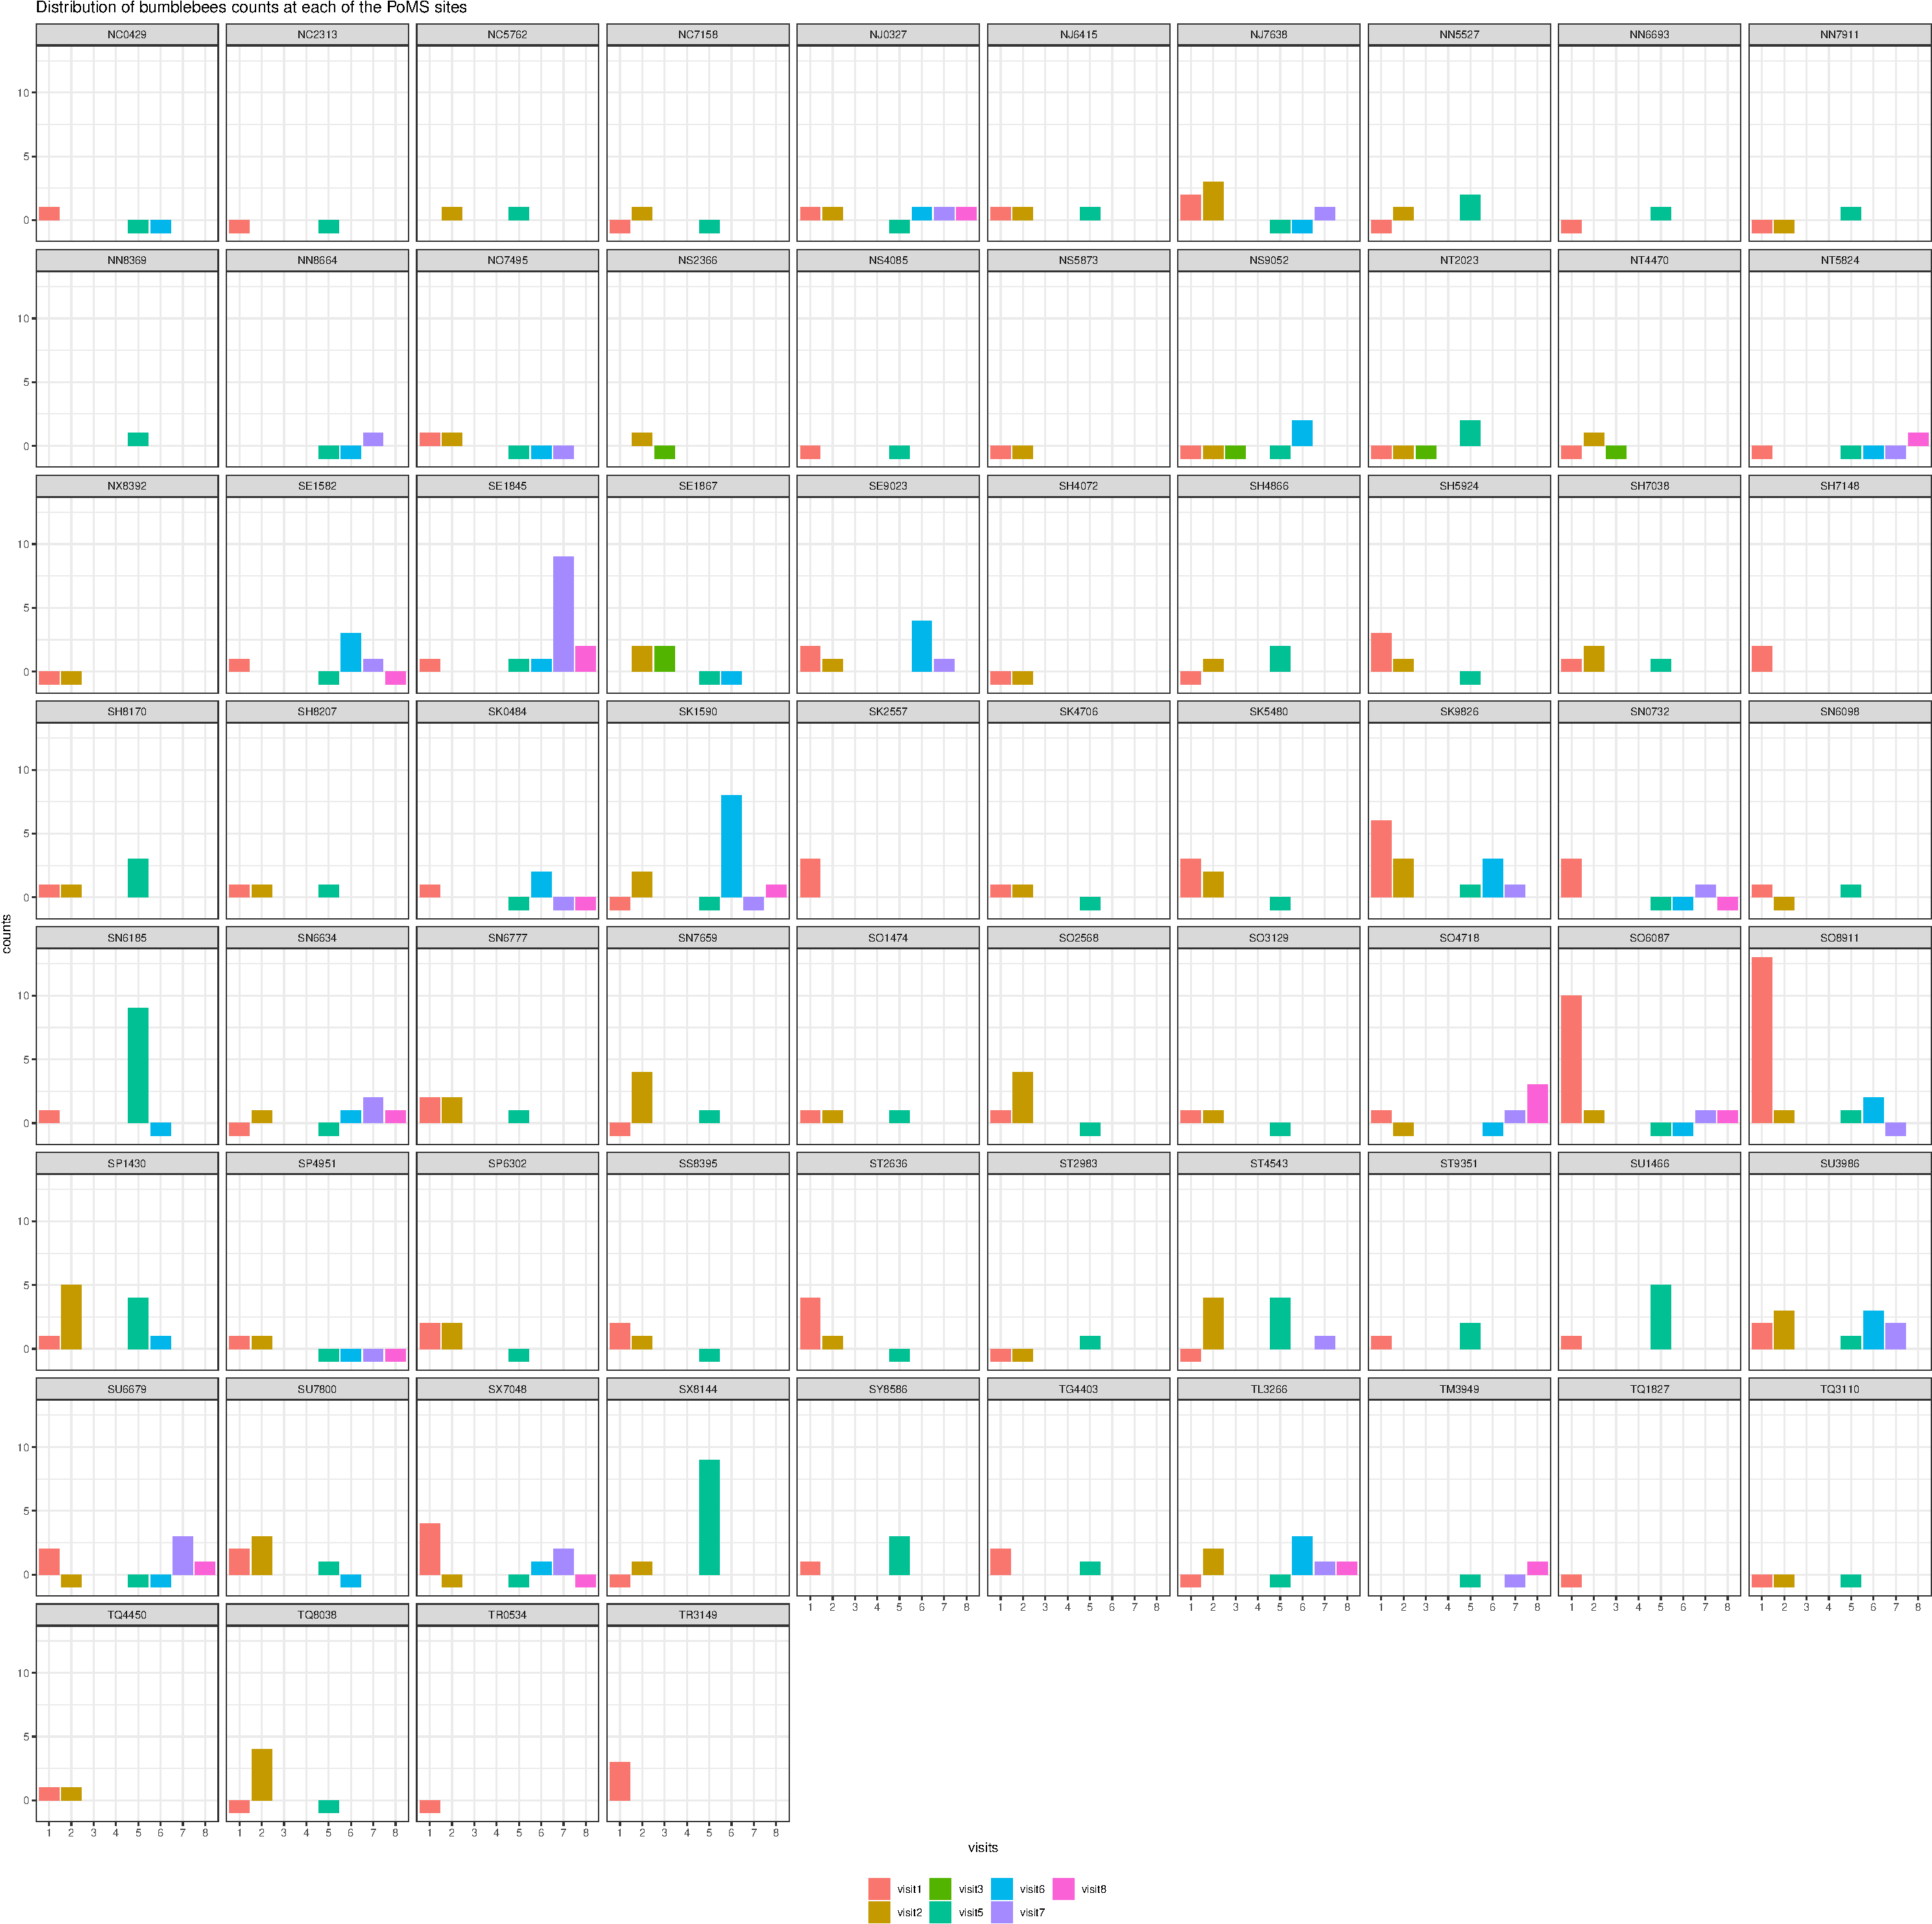
\includegraphics{SupplementaryInformationOne_files/figure-pdf/fig-bbGCPlot-1.pdf}

}

\caption{\label{fig-bbGCPlot}Distribution of bumblebess counts for the
74 PoMS sites. The counts are facetted by the PoMS site name and colored
by the visit number the observations was made. The columns of visits
without no bars represent the visit without no group count obervation
(`NA').}

\end{figure}

\begin{figure}

{\centering 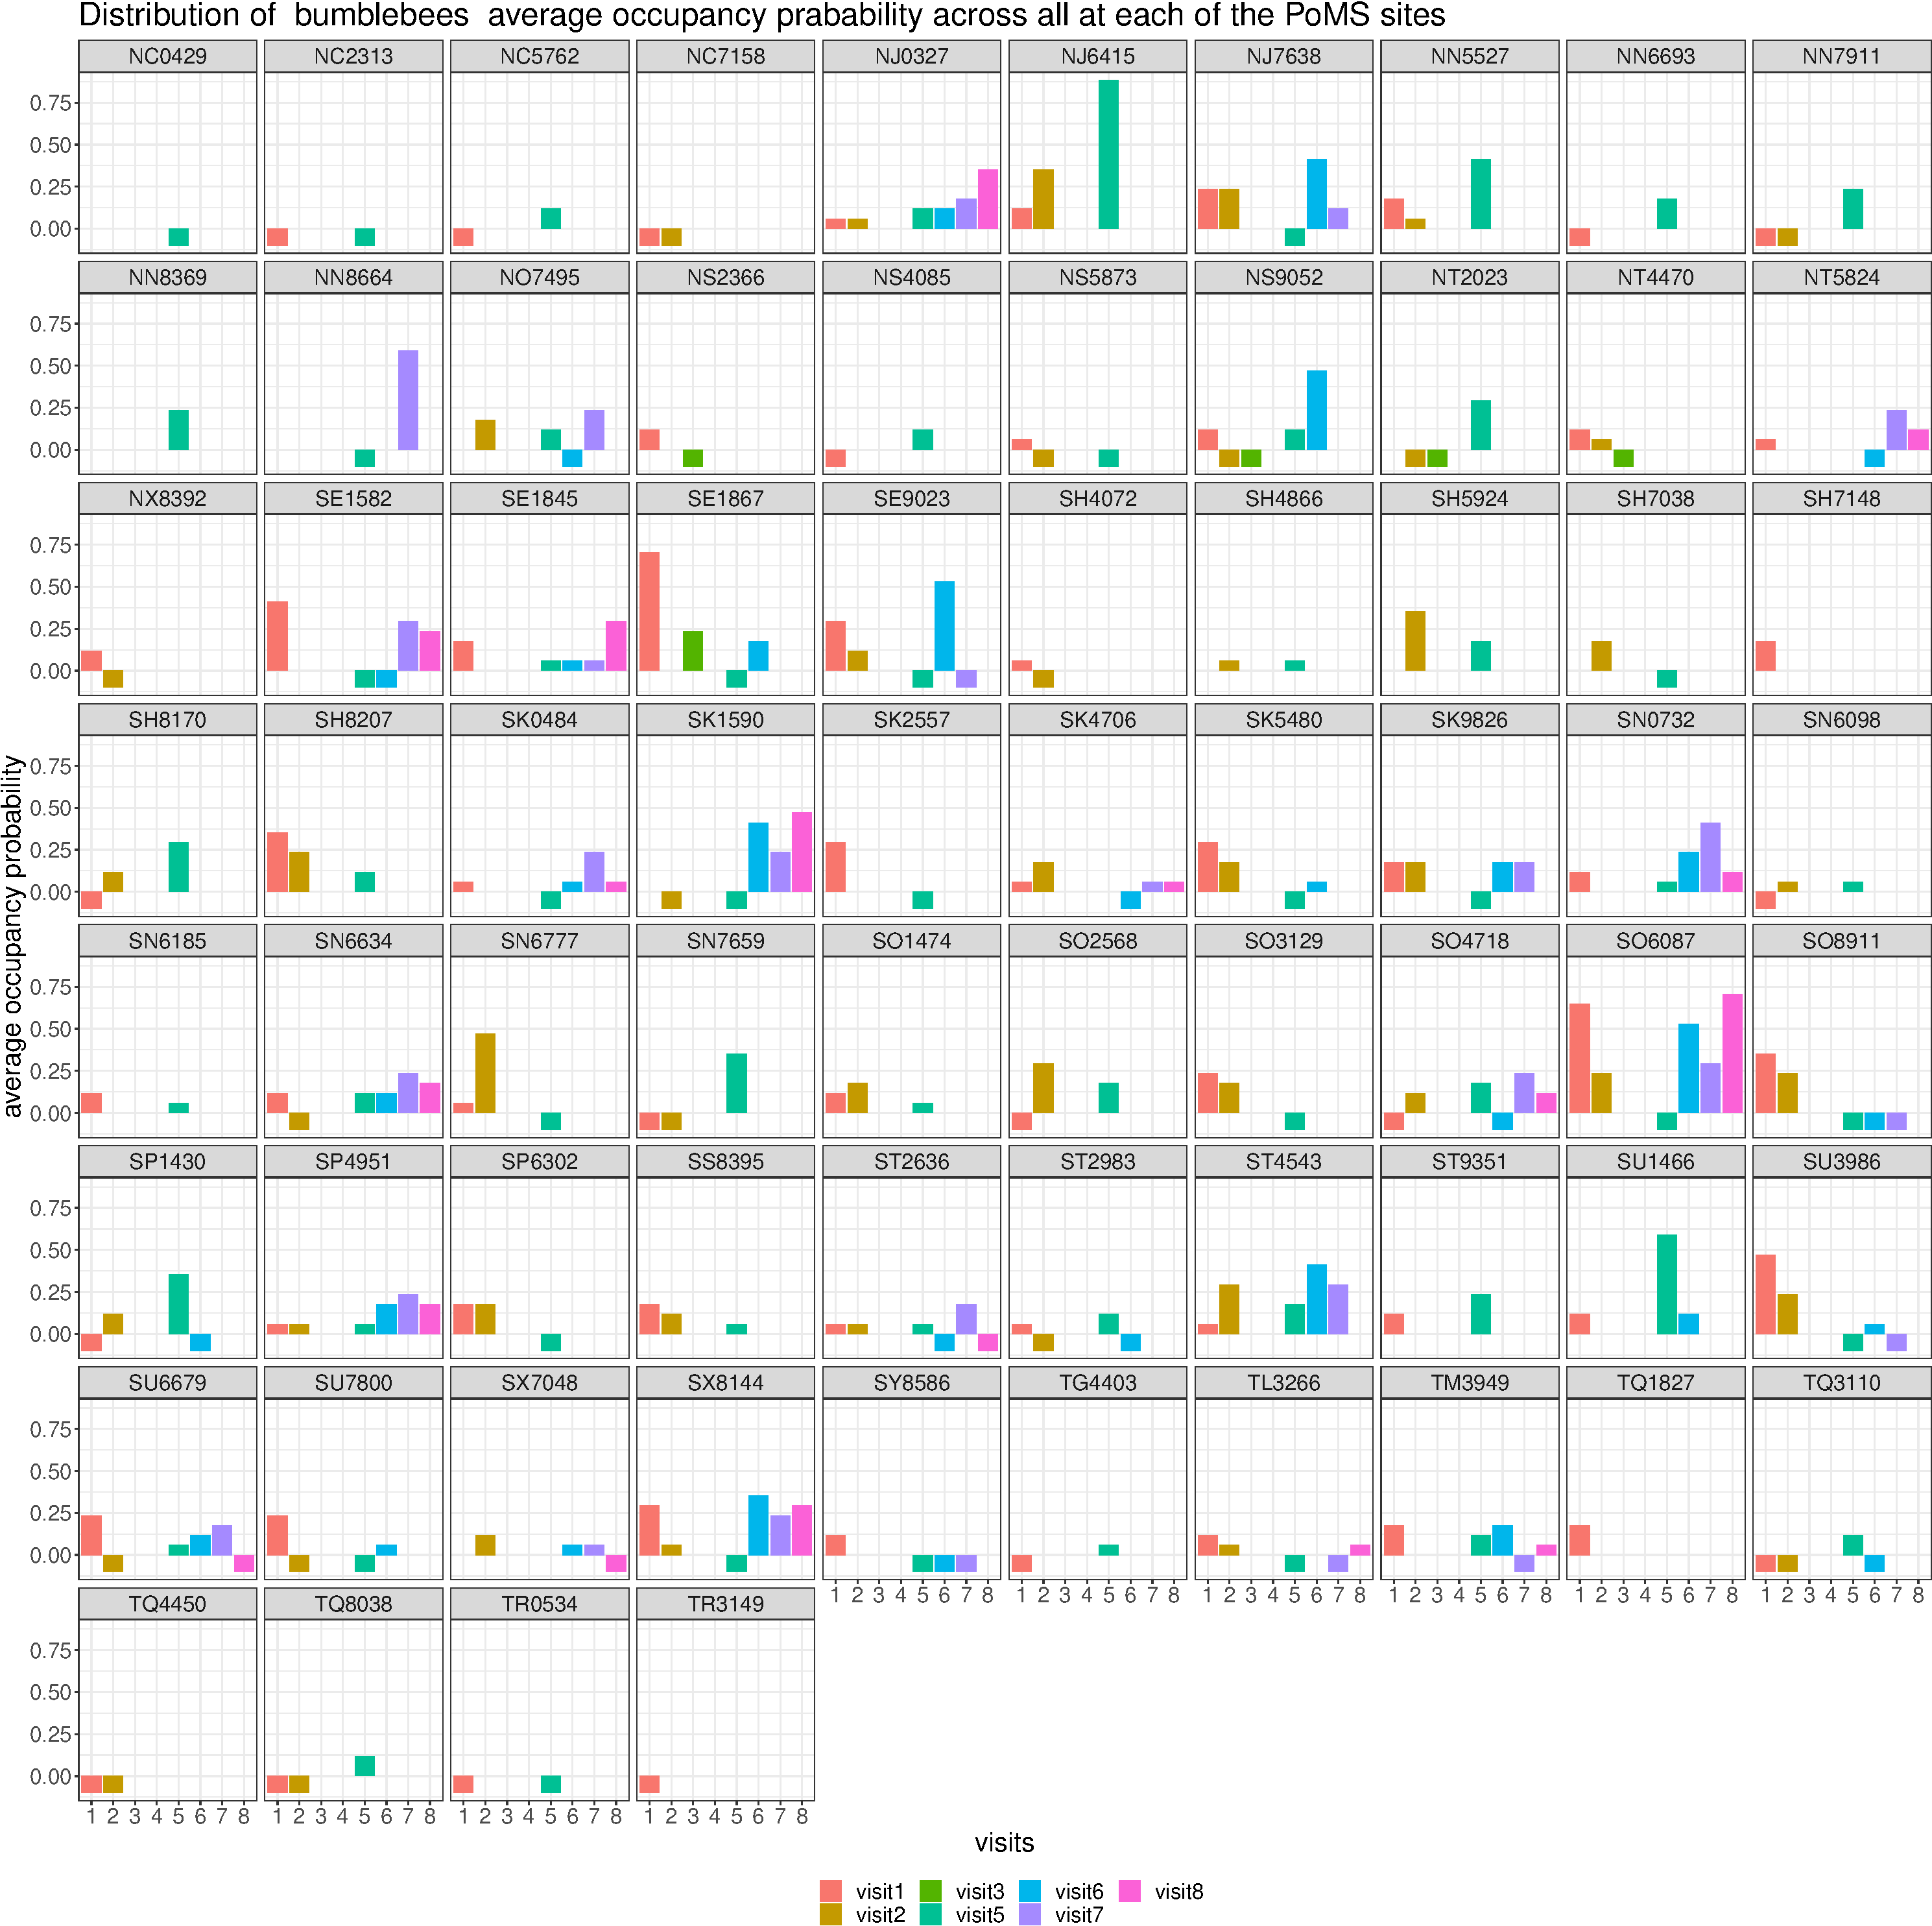
\includegraphics{SupplementaryInformationOne_files/figure-pdf/fig-bbSOPlot-1.pdf}

}

\caption{\label{fig-bbSOPlot}Distribution of bumblebees occupancy
probability for the 74 PoMS sites. The probabilities for each site are
estimated as the proportion of sites with at most one pantrap being
occupied by the species. The occupancy probabilities are facetted by the
PoMS site name and colored by the visit number the observations was
made. The columns of visits without no bars represent the visit without
no group count obervation (`NA').}

\end{figure}

\begin{figure}

{\centering 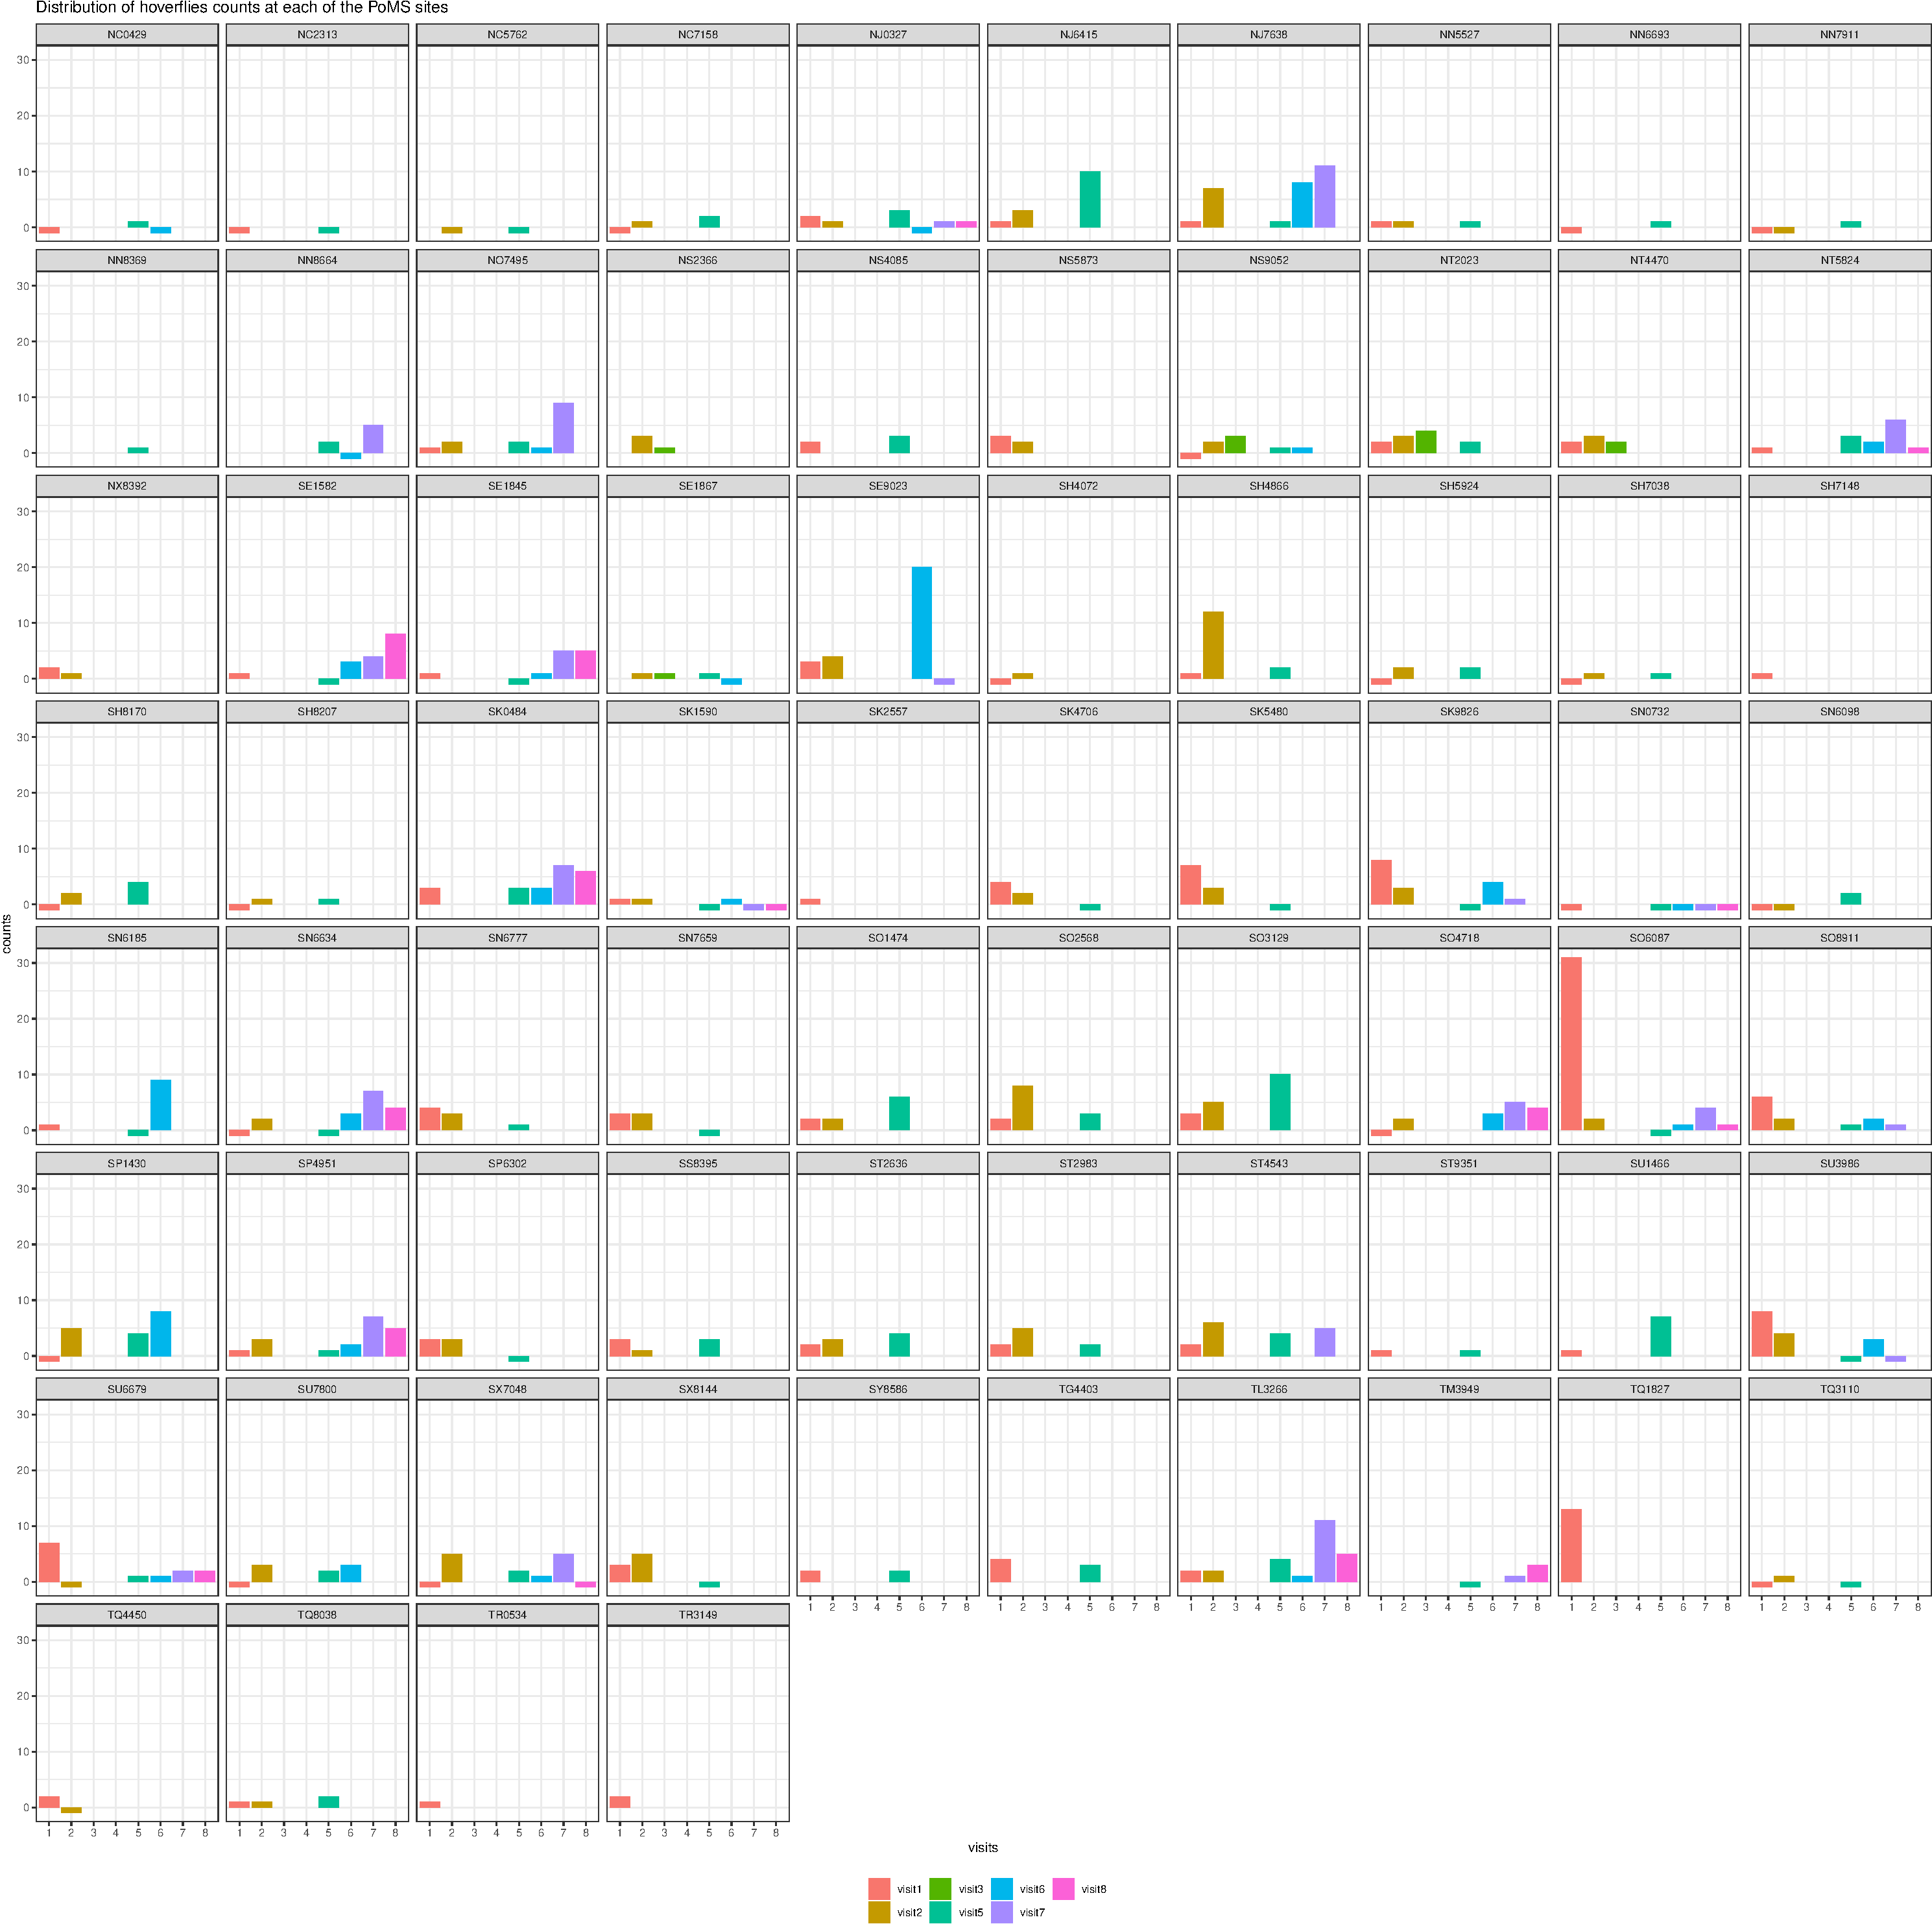
\includegraphics{SupplementaryInformationOne_files/figure-pdf/fig-hvGCPlot-1.pdf}

}

\caption{\label{fig-hvGCPlot}Distribution of hoverflies counts for the
74 PoMS sites. The counts are facetted by the PoMS site name and colored
by the visit number the observations was made. The columns of visits
without no bars represent the visit without no group count obervation
(`NA').}

\end{figure}

\begin{figure}

{\centering 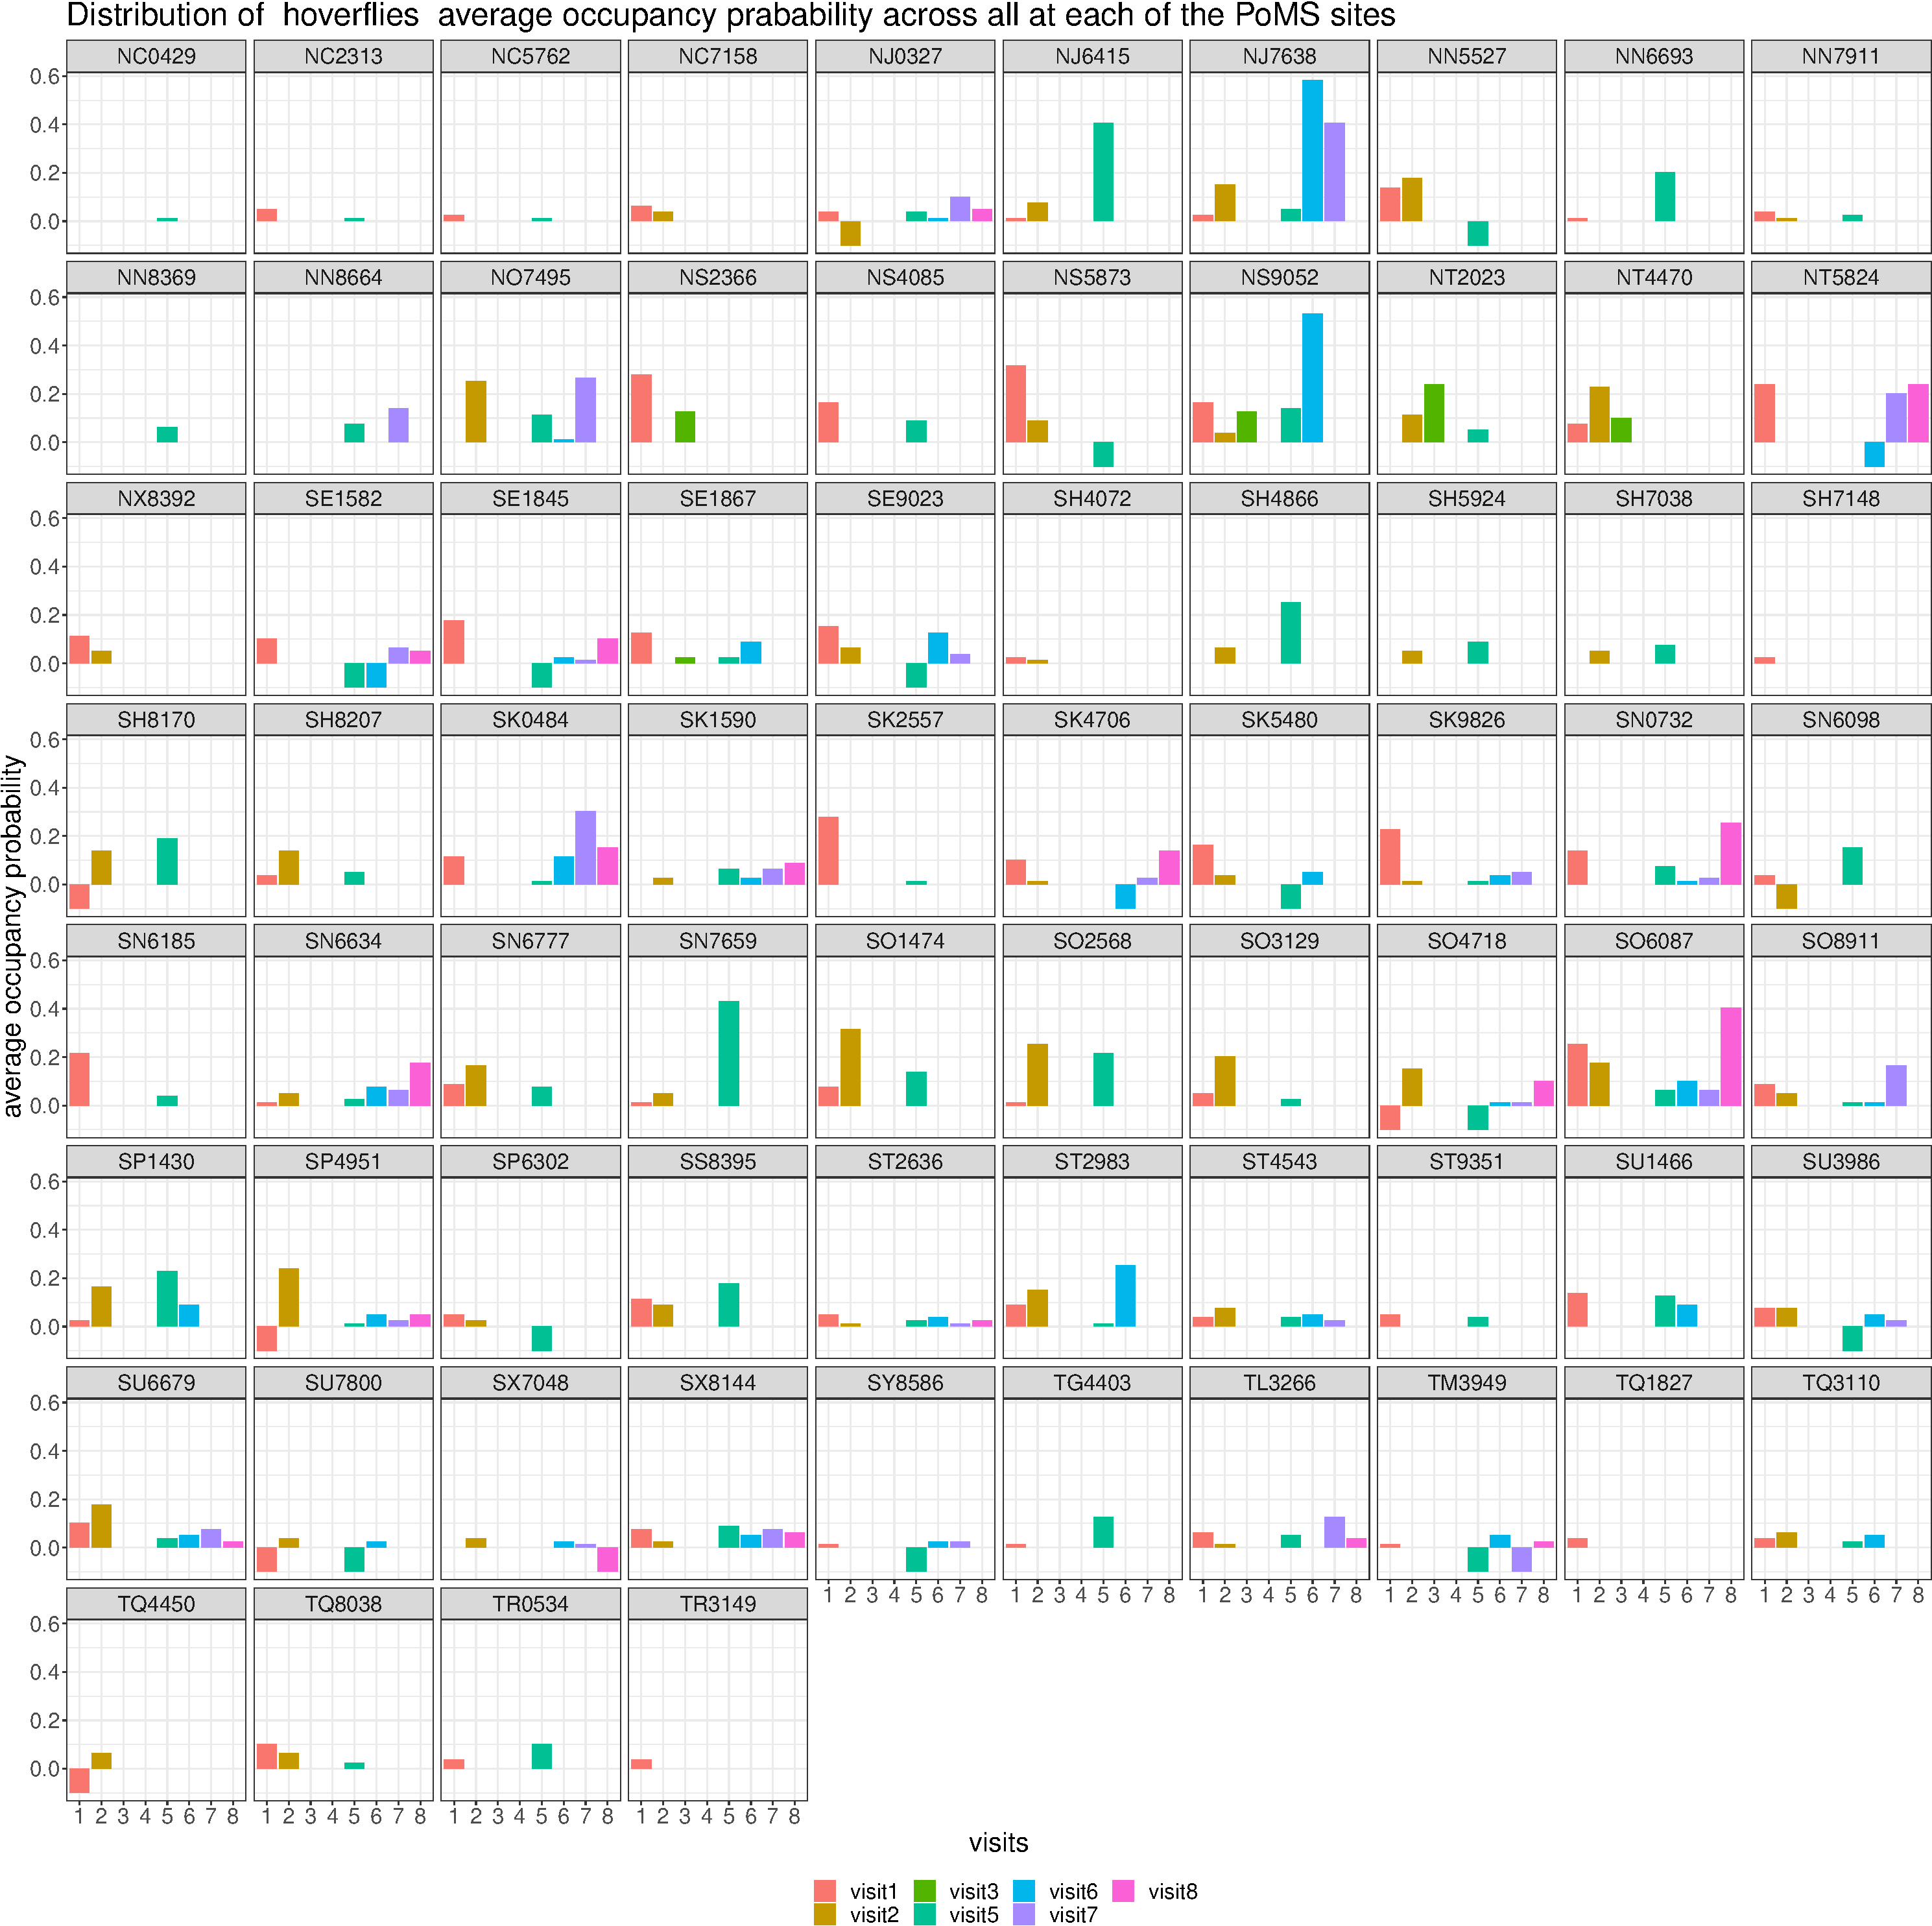
\includegraphics{SupplementaryInformationOne_files/figure-pdf/fig-hvSOPlot-1.pdf}

}

\caption{\label{fig-hvSOPlot}Distribution of hoverflies occupancy
probability for the 74 PoMS sites. The probabilities for each site are
estimated as the proportion of sites with at most one pantrap being
occupied by the species. The occupancy probabilities are facetted by the
PoMS site name and colored by the visit number the observations was
made. The columns of visits without no bars represent the visit without
no group count obervation (`NA').}

\end{figure}

\begin{figure}

{\centering 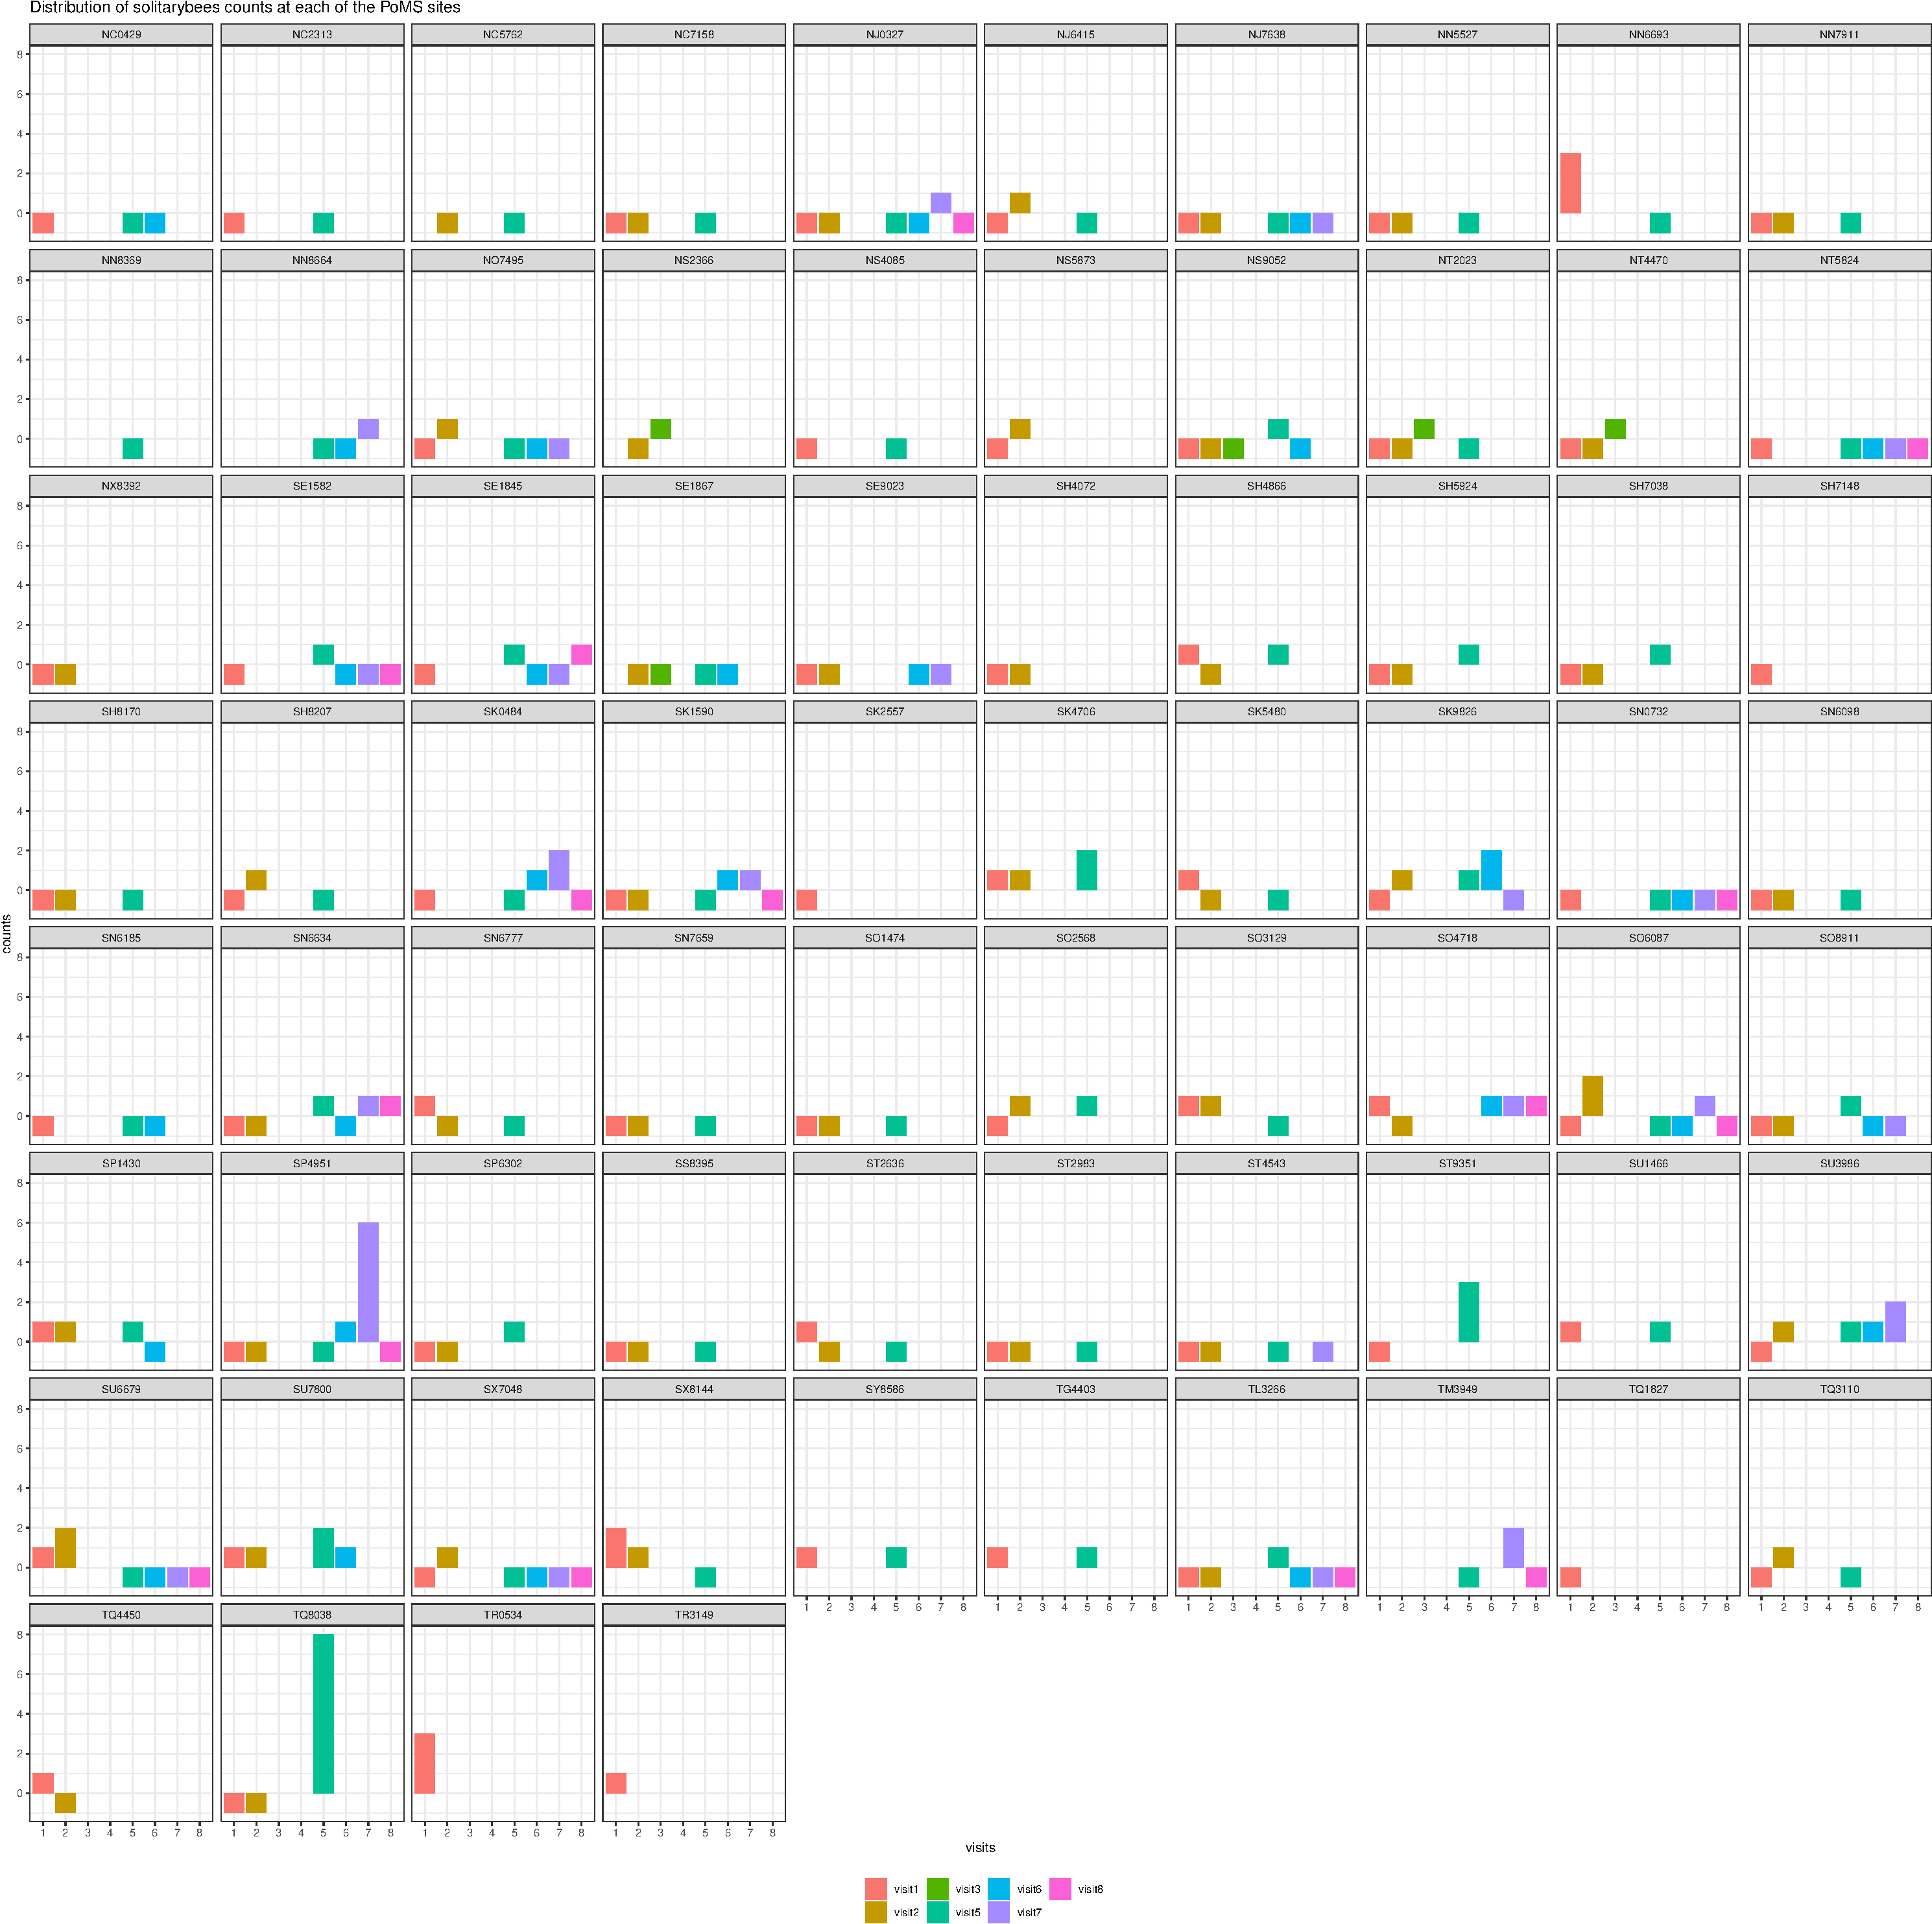
\includegraphics{SupplementaryInformationOne_files/figure-pdf/fig-sbGCPlot-1.pdf}

}

\caption{\label{fig-sbGCPlot}Distribution of solitarybees counts for the
74 PoMS sites. The counts are facetted by the PoMS site name and colored
by the visit number the observations was made. The columns of visits
without no bars represent the visit without no group count obervation
(`NA').}

\end{figure}

\begin{figure}

{\centering 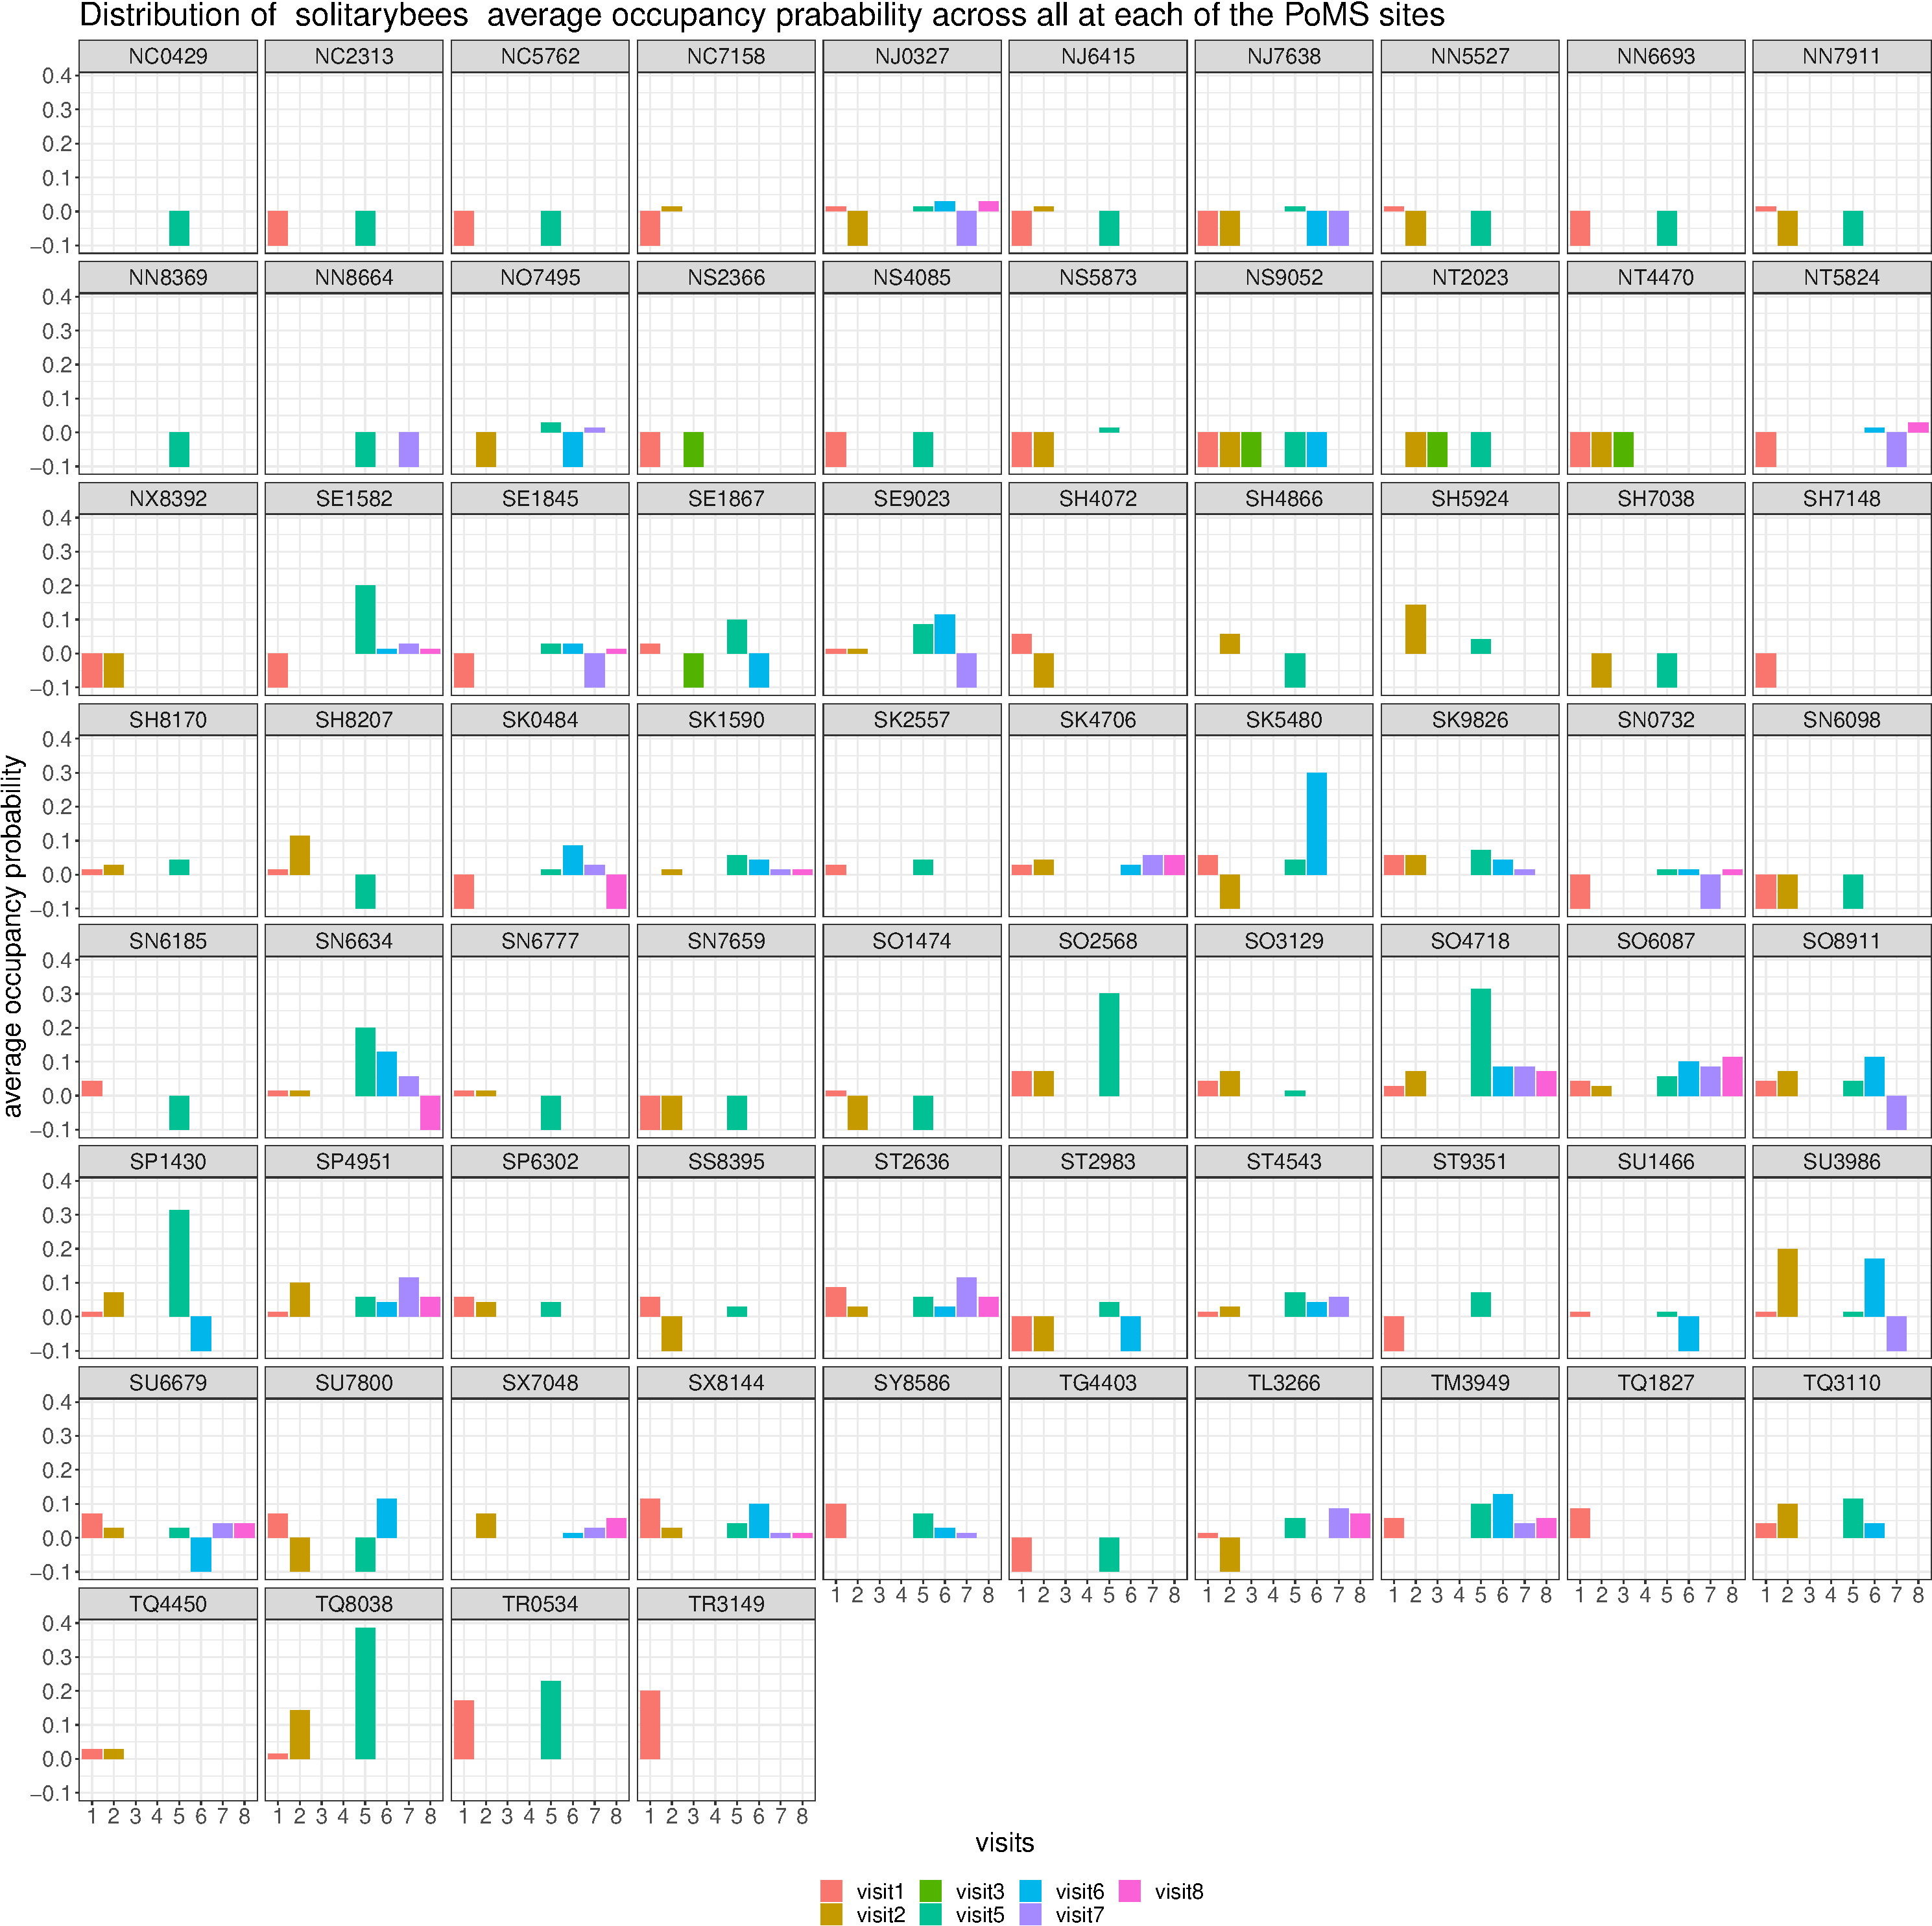
\includegraphics{SupplementaryInformationOne_files/figure-pdf/fig-sbSOPlot-1.pdf}

}

\caption{\label{fig-sbSOPlot}Distribution of solitarybees occupancy
probability for the 74 PoMS sites. The probabilities for each site are
estimated as the proportion of sites with at most one pantrap being
occupied by the species. The occupancy probabilities are facetted by the
PoMS site name and colored by the visit number the observations was
made. The columns of visits without no bars represent the visit without
no group count obervation (`NA').}

\end{figure}

\hypertarget{combining-both-datasets}{%
\subsection{Combining both datasets}\label{combining-both-datasets}}

From the results and discussions above, we model the group count with a
negative binomial GLMM with latitudinal gradient as a covariate and
visit random effect. The species occupancy probabilities were modeled
with a binomial GLMM with latitudinal gradient as a covariate and
species and visit random effect. We allow both models to share
latitudinal gradient effect as well as species and visit random effects.
The details are describe under section \(2.2\) in the main paper.

\hypertarget{references}{%
\subsubsection{References}\label{references}}

\renewcommand{\bibsection}{}
\bibliography{references.bib}




\end{document}
